\chapter{\textsc{Généralités}}\label{generalite}
Pour mieux aborder ce sujet, il est essentiel d'avoir une compréhension globale des lubrifiants et du système (circuit) de lubrification des moteurs. Ce chapitre sera structuré en deux grandes parties, permettant une analyse claire et progressive.

Dans un premier temps, nous nous concentrerons sur la nature et les caractéristiques des lubrifiants. Cela inclura leur processus de production, les différents types existants, leurs applications dans des contextes variés, ainsi que les impacts environnementaux liés à leur utilisation. Une attention particulière sera portée aux défis actuels et aux innovations visant à réduire l'empreinte écologique des lubrifiants.

Dans un second temps, nous explorerons le système SPC (Segment-piston-cylindre) en détaillant le circuit de lubrification, son rôle dans l'amélioration du rendement moteur, ainsi que les spécificités de sa lubrification. Une analyse approfondie des interactions entre le système SPC et les performances mécaniques permettra de mieux comprendre son importance dans les moteurs modernes.

\section{\textsc{Généralité sur la Lubrification}}\label{lubrification}
Il serais tout de même naturel avant de plonger dans notre étude sur la \textbf{lubrification}, de bien vouloir en parler quelque soit peu, en vue de donné quelques bases au lecteur pour la suite; ainsi nous allons définir la lubrification, donné quelques sortes et insister sur ce qui nous intéresse, parler de l'utilisation  passant par certaines caractéristiques de Lubrifiants.

\subsection{Lubrifiant Moteur}
Le lubrifiant se met entre les surfaces en mouvement relatif afin d'éviter le contact solide entre elles, limiter le frottement et, par conséquent, assurer le bon fonctionnement des mécanismes. Il peut être solide, liquide ou gazeux. Les lubrifiants destinés à la lubrification des MCI sont généralement liquides. C'est sur cette catégorie que porte l'étude dans le présent travail.\\

D’un point de vue technologique, le lubrifiant assure plus que son simple rôle de réduction de frottement, il faut aussi tenir compte des propriétés thermodynamique(un rôle de liquide refroidissement), la protection contre l'usure chimique, la repartition de la pression dans certain cas l'evacuation de debris. Le contrôle de telles propriétés est géré par le type de lubrifiant et certains additifs qui entrent dans sa composition. Mais la fonction essentielle d’un lubrifiant réside dans sa capacité à réduire les pertes d’énergie mécanique par frottement afin d’améliorer le rendement.\\

Pour ce faire, Les lubrifiants sont alors composés majoritairement d’une huile de base, à laquelle sont ajoutés des additifs. La teneur de ces derniers est généralement faible, de l’ordre de 5$\%$ de la masse totale du lubrifiant, mais peuvent atteindre parfois des proportions beaucoup plus importantes (plus de 25$\%$) selon les applications auxquelles le lubrifiant est destiné\cite{Amal}

\subsection{Les Huiles Lubrifiants}
De par leur composition chimique et leur provenance, les huiles peuvent être classées en deux familles principales : minérales et synthétiques, Il y a également des huiles de bases végétales qui ne sont pratiquement pas utilisées dans l’industrie automobile.\cite{initiation}

\subsubsection{Les huiles minérales}
Provenant du pétrole, les huiles sont extrait de la distilation du petrole brute.Ces coupes subissent des opérations de raffinage dont la complexité dépend à la fois de l’origine du brut utilisé et de la qualité recherchée des produits
\begin{itemize}
	\item Les huiles paraffiniques sont composées d’hydrocarbures saturés linéaires (n-paraffines) ou ramifiés (isoparaffines). Ils ont une bonne stabilité à l’oxydation et un indice de viscosité élevé
	(plus que 60 SSU\footnote{SSU (Second Saybolt Universal) est l'ancien système d'unité empirique de la viscosité.}). Leur pouvoir solvant est par contre limité (indice S ou NS pour Solvant ou Neutral Solvant) et leur point de congélation élevé. Les isoparaffines peuvent avoir un point de
	congélation moins élevé, mais présentent un plus faible indice de viscosité.
	\item Les huiles naphténiques sont composées d’hydrocarbures saturés cycliques. Contrairement à
	la catégorie précédente, ils sont moins stables à l’oxydation, possèdent des indices de viscosité
	plus faibles (moins que 60 SSU), mais ont un grand pouvoir solvant et possèdent de meilleures
	caractéristiques d’écoulement à basse température.
\end{itemize}

\subsubsection{Les huiles synthétique}
Les huiles minérales présentent des limitations (notamment une forte dépendance de la viscosité à la température) qui a conduit au développement d’huile plus performantes dites de synthèse. Leur obtention nécessite un processus chimique qui est généralement beaucoup plus coûteux que la distillation et le raffinage. Les composants utilisés dans la composition de ces huiles proviennent de la pétrochimie, carbochimie, lipochimie et de la chimie minérale (oléphines aromatiques, alcools, acides,composés halogénés, phosphorés, silicatés, …). Cette famille d’huiles présent de meilleures performances que la famille des huiles à base minérale en terme de tenue thermique, résistance à l’oxydation et indice de viscosité

\subsection{Les Additifs}\label{additifs}
Les performances des lubrifiants sont généralement améliorées grâce à l’ajout d’additifs.Ils en existent de plusieurs sortes des produits organiques, minéraux ou organométalliques qui agissent chimiquement ou physiquement à différents niveaux pour assurer plusieurs fonctions, selon l’utilisation à laquelle un lubrifiant est destiné et les conditions de fonctionnement. Sans être exhaustif, nous enumérons quelques propriétés additifs, notamment celles qui concernent les huiles utilisées dans la lubrification des MCI.\cite{initiation}\\

\begin{table}[h!]
	\begin{tabular}{ l l l }
		\hline
		\multicolumn{3}{c}{Point de vu chimie} \\
		\hline
		\textbf{Additifs}	&\textbf{Rôles}  			    &\textbf{Mode de fonctionnement}  \\
		\hline
		Anti-usure	&Réduire l’usure et le frottement&Ces additifs réagissent chimiquement avec \\
		&prévenir du grippage.			 &la surfacemétallique pour former un film \\
		&						&sacrificiel présentant une résistance au \\
		&						&cisaillement plus faible que le métal.  \\
		\hline
		Anticorrosion&Empêcher la corrosion des surfaces. &  Formation d’un film adsorbé sur la surface qui\\
		&								   &protège de la corrosion.\\
		\hline
		Antioxydation&Empêcher l’oxydation du lubrifiant.  &Décompose les composants (hydroperoxydes)\\
			&&qui conduisent à l’oxydation des huiles  \\
		\hline
		Antimousse&Empêcher la formation&Réduit la tension de surface du lubrifiant pour	\\
		&de mousse dans le lubrifiant  &faciliter le destruction des bulles d’air.  \\
		\hline
		\multicolumn{3}{c}{Point de vu Physique} \\
		\hline
		Amélioration de & d’améliorer la viscosité&Ils épaississent le lubrifiant et réduisent \\
		l’indice de viscosité& à haute température 	&la chute de viscosité observée à chaud,\\				
		\hline
		Abaissement du point &d'abaisser le point de &perturbant le processus de cristallisation\\
		d’écoulement & température où l’huile peut couler & des paraffines dans l’huile de base.  \\
		\hline
	
	
	\end{tabular}
	\label{tab:additifs}
	\caption{Tables des Additifs et leur rôles \cite{initiation}}
\end{table}

\subsubsection{Comportement Tribologique de MoDTC et ZDDP}
Il nous est parue important de parler un peu plus dans l'exposer sur le dithiocarbamate de molybdène (MoDTC) et le dithiophosphate de zinc (ZnDTP ou ZDDP). ces additifs sont les plus utliser comme nous allons le voir plus loin. En effet, on peut distinguer entre la fonction de réduction de frottement, assurée le plus souvent par le MoDTC et la réduction de l’usure assurée majoritairement par le ZDDP.\\

La courbe typique de l'évolution du frottement associée au MoDTC est représentée par la (la figure \ref{fig:modtc-et-friction})Une nette diminution du frottement peut être observée en présence de l'additif MoDTC dans le lubrifiant. Le frottement est élevé au début de l'essai puis il chute à des valeurs faibles et stables. Le temps nécessaire pour que le frottement diminue entre le début de l'essai et le régime stationnaire
correspond à l'activation de la molécule MoDTC. Il est appelé temps d'induction. Le coefficient de frottement dans des conditions du régime limite peut être aussi faible que 0.04\cite{Amal}
\begin{figure}[h]
	\centering
	\includegraphics[width=0.7\linewidth]{"Img/MoDTC et friction"}
	\caption[]{Evolution de la friction avec MoTDC et sans MoDTC}
	\label{fig:modtc-et-friction}
\end{figure}

La (figure \ref{fig:zddp-evolution}) représente le facteur d'usure qui indique l'efficacité du lubrifiant dans la réduction de l'usure. En comparant avec l'huile de base et les autres lubrifiants contenant le MoDTC, l'usure
la plus faible est observée dans le test où le ZDDP est ajouté au lubrifiant. On peut également remarquer que la présence du MoDTC, c'est-à-dire le lubrifiant 003A, a un effet réducteur d'usure. Coefficient d'usure en fonction des lubrifiants, mesuré après 6 heures de frottement à 100 °C, vitesse de glissement de 0.1 m/s et une charge de 188 N.
\begin{figure}[h]
	\centering
	\includegraphics[width=0.7\linewidth]{"Img/Zddp evolution"}
	\caption[]{Histogramme comparatif entre le ZDDP et MoDTC}
	\label{fig:zddp-evolution}
\end{figure}

nous tennons à preciser que la La bibliographie présentée ci-haut fait référence aux tests de frottement menés dans de contacts acier/acier lubrifiés en régime limite avec des huiles contenant la molécule MoDTC et la molécule ZDDP.

\subsection{Les Revêtements de surface}
Les revêtements sont aujourd'hui de plus en plus employés pour améliorer les caractéristiques tribologiques telles que le frottement et la résistance à l'usure des surfaces en mouvement relatif. Il s'agit de déposer une ou plusieurs couches d'un matériau (ou plusieurs matériaux) sur les surfaces en contact. Les revêtements fréquemment utilisés dans le domaine automobile sont le chromage $CrN$, dépôt des couches minces de carbone amorphe DLC (Diamond-like carbon), dépôt des couches de nanoparticules du MoS2 (bisulfure de molybdène) et des couches de WS2 (bisulfure de tungstène).\cite{Amal}\\

Dans certains environnements extrêmes, il n’est pas possible d’utiliser des lubrifiants fluides. C’est le cas d’applications cryogéniques, d’applications à très haute température ou dans l’espace. On fait alors appel à des lubrifiants solides. Ils sont déposés en couches entre les solides en frottement et jouent le rôle d’un troisième corps qui peut se cisailler facilement pour réduire le frottement et limiter l’usure.

Nous ne pouvons guère entrer plus loin dans les revêtement étant donner que notre étude est basée sur le les huiles de lubrification et non dans le revêtement car il y a un monde derriere ce type de lubrification.
\subsection{Impacte de lubrifiant moteur dans la nature}
Les lubrifiants issus du pétrole posent des problèmes environnementaux majeurs, principalement en raison de leur faible biodégradabilité, de leur toxicité, et de leur potentiel à polluer les sols, les eaux, et l’air. La contamination des sols et des eaux : Les lubrifiants pétroliers, lorsqu'ils sont mal éliminés ou rejetés accidentellement, infiltrent les sols et contaminent les eaux souterraines. Cela entraîne une diminution de la qualité des sols et affecte la biodiversité environnante\cite{enveroile}\\

Le ZDDP et le MoDTC comme vue plus haut(partie\ref{additifs}), sont des additifs principales pour renforcer les qualités des lubrifiants de base. néanmoins, ils sont tout aussi polluant. Lorsque ZDDP est rejeté dans l’environnement, il libère des composés de zinc et de phosphore, qui peuvent contaminer les sols et les eaux.Le phosphore contribue à l’eutrophisation des cours d’eau, entraînant une prolifération d’algues et une diminution de l’oxygène disponible pour la faune aquatique.Les particules de zinc, en concentration élevée, peuvent être toxiques pour les organismes vivants, affectant les plantes et les animaux.\cite{zddp} Quant au MoDTC L'accumulation de molybdène dans les sols et les eaux peut être nocive, bien que ses effets écotoxicologiques soient moins connus que ceux du phosphore ou du zinc. Les études indiquent également que le MoDTC peut se dégrader thermiquement, produisant des sous-produits qui augmentent la corrosivité des lubrifiants.\cite{zddp}\\
 
Face à cette problématique, des recherches se concentrent sur le développement de lubrifiants issus de matières végétales ou synthétiques, qui permettent de réduire significativement l’impact environnemental. Cependant, il convient de noter que même les huiles dites biodégradables peuvent contenir jusqu’à $50\%$ de composés d’origine pétrolière, limitant ainsi leur véritable efficacité écologique.\cite{enveroile}\\

En conclusion, bien que les lubrifiants pétroliers soient encore largement utilisés, leur impact environnemental nécessite une transition vers des alternatives plus respectueuses, accompagnée de réglementations plus strictes et d’initiatives de recyclage globales.
%% SECTION DE LA VU D'ENSEMBLE DE SPC
\section{\textsc{Vue d'ensemble du système Segmentation-Piston-Chemise et état de l'art} }\label{spc}
Le système de segmentation, piston et chemise (SPC) est au cœur de la performance d’un moteur, où les segments joue certains rôles garantissant l’étanchéité et la dissipation de la chaleur tout en minimisant les pertes par frottement. Cette section présente une vue d'ensemble de ce système ainsi qu’un état de l’art, en explorant l’évolution des techniques et matériaux utilisés pour la lubrification et la réduction de frottement.
\subsection{Moteur à combustion interne}
Le système SPC dans le cadre de notre travail est employée dans le moteur à combustion interne, il est ainsi naturelle de définir le moteur et de parler de son fonctionnement.\\

Le moteur à combustion interne peut être défini comme un convertisseur de l'énergie chimique (la chaleur) contenue dans le fluide de travail en énergie mécanique ici recueilli dans le couple de l'arbre moteur. Nous allons donc en distinguer deux sortes : moteur à apport de chaleur externe et moteur à combustion interne.\cite{sumuna}
\begin{figure}[h]
	\centering
	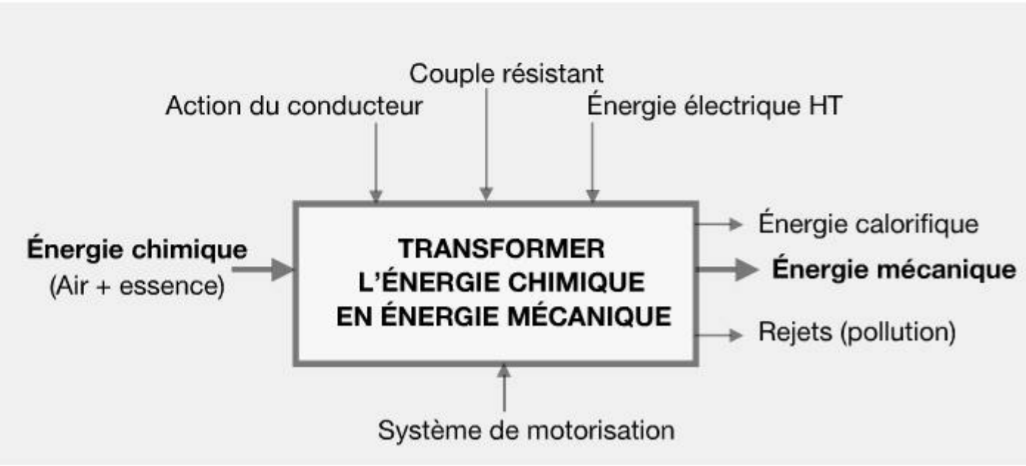
\includegraphics[width=0.7\linewidth]{Img/convertisseur}
	\caption[Convertisseur]{Convertisseur d'énergie thermique en mécanique}
	\label{fig:convertisseur}
\end{figure}
Nous  distinguons deux types des moteurs dans la famille de moteur à combustion interne, nous pouvons citer :
\begin{itemize}
	\item Moteur à explosion (à essence) dans lequel la combustion du mélange aire - carburant est amorcée par l'étincelle d'une bougie d'allumage. Ils possèdent donc un système d'allumage commandé.\cite{tecauto}
	\item Moteur à combustion interne (Diesel) dont la combustion est déclenchée par l'injection des gaze sous pression dans de l'aire fortement comprimé. il se produit une auto - inflammation.\cite{tecauto}
\end{itemize}
Tous les moteurs à combustion interne à mouvement alternatif se comporte de la même manière; on y trouve essentiellement les mêmes éléments comme le montre la (figure \ref{fig:partie-du-moteur}) : La \textbf{chambre de combustion} qui est un volume ou pénètrent et réagissent les gaz; le \textbf{cylindre}, qui est le prolongement de la chambre de combustion; le \textbf{piston}, qui se déplace dans le cylindre et fait varier le volume de la chambre de combustion; le \textbf{Système bielle - manivelle}, qui est solidaire, à une extrémité, du piston et, à l’autre, du \textbf{vilebrequin}, et qui transforme le mouvement de va-et-vient du piston en un mouvement de rotation. le \textbf{bloc-moteur}, qui constitue l’enveloppe mécanique de l’ensemble.\cite{approche}\\

\begin{figure}[h]
	\centering
	\includegraphics[width=0.5\linewidth]{"Img/partie du moteur"}
	\caption[Partie du moteur]{Partie du moteur}
	\label{fig:partie-du-moteur} \cite{approche}
\end{figure}

\subsection{Description du Segment}
Les segments sont des anneaux brisés, de section carrée ou parallélépipédique, travaillant en extension. Ils doivent assurer des pressions radiales uniformes sur les parois du cylindre. La fonte douce qui les compose reçoit un chromage évitant une usure rapide par frottement. Leur position dans les gorges permet à la pression des gaz d'accentuer leur étanchéité.\cite{tecauto} Ils peuvent être au nombre de 2,3 ou 4 allant jusqu'à 5 sur les grands moteurs diesels suralimentés cela dépend du diamètre du piston. La fonction primaire de la segmentation est d'empêcher les fuites de gaz entre le piston et la chemise.Cependant, sans lubrification, ce contact étroit entre le segment et la chemise aurait comme conséquence de grandes pertes de puissance par frottement.En conséquence, l'autre objectif principal des segments est de distribuer efficacement le lubrifiant le long de l'interface segment/chemise, sans permettre à l'huile excessive de passer l'interface et de fuir vers la chambre de combustion où il pourrait être brulé.Une troisième fonction des segments qui est particulièrement importante pour le segment supérieur est la dissipation de la chaleur du piston vers le cylindre, comme montre la (figure \ref{fig:partie-du-segment}).\\

\begin{figure}
	\centering
	\includegraphics[width=0.5\linewidth]{"Img/partie du segment"}
	\caption[Segmentation]{Segmatation}
	\label{fig:partie-du-segment}
\end{figure}


Afin que ce système puisse atteindre efficacement ces objectifs globaux, chaque segment a un rôle unique. Le segment de dessus \textbf{coup de feu} scelle l'interface segment/chemise afin d'empêcher le gaz à haute pression de s'échapper de la chambre de combustion vers le carter (Blow by)\footnote{Dans un moteur, le blow-by est une fuite de gaz de combustion qui s'échappe des cylindres vers le carter d'huile}. Le segment \textbf{racleur} règle la quantité d'huile qui passe du carter pour lubrifier les segments supérieurs. Un deuxième segment est également présent dans la plupart des moteurs \textbf{segment d’étanchéité}, ce segment érafle en bas l'huile excessive qui passe l'interface segment racleur d'huile/chemise et vient en aide au premier segment affin de chasser le reste des gaz fuyards. La deuxième interface segment \textbf{d’étanchéité/chemise} fournit ainsi une barrière contre l'écoulement d'huile dans la gorge supérieure, et des gaz pour les parties plus inférieures du piston, ce qui réduit la consommation d’huile. \cite{ayad1}\\

le segment \textbf{coup de feu} c’est le segment qui est soumis aux plus fortes températures :une temperature pouvant se levée jusqu'à $250\degres C$. Ainsi il faut trouver le bon compromis thérmodynamique et de géométrie pour eviter le risque de matage\footnote{Le matage est une déformation plastique localisée de la matière sous l'effet d'un choc ou d'une pression élevée.},une faible épaisseur donc une faible surface de contact, diminuant les échanges thermiques, et une faible masse permettant des fonctionnements à des régimes plus élevés. Le segment coup de feu est généralement revêtu d’une couche de chrome ou de molybdène.\cite{technologie1}.\\

Le segment d’\textbf{étanchéité} peut également être un segment rectangulaire mais on trouve souvent : la portée du segment sur une arête lui confère une grande efficacité pour le raclage de l’huile, il existe aussi le segment à bec d’aigle qui est bien placé pour la consommation d'huile et pour finir nous le segment à chanfrein de torsion:ce type de segment permet d’assurer le contact sur une arête\cite{technologie1}\\

Il est impératif de prévoir à l’arrière du segment racleur des passages par lesquels l’huile va pouvoir s’écouler (trous en fond de gorge ou embrèvements dans la partie inférieure de la gorge\\), pour remplir cette fonction, le segment est conçu avec une certaine technologie qui est different aux autres:Segment racleur à ressort spiroïdal dont les lèvres peuvent être chromées ou non suivant la pression de contact; les segment racleur à deux rails d’acier; le segment UFLEX dont a un problème principal  est sa difficulté de montage liée à sa grande longueur à vide. Son principal avantage est son faible coût. \cite{technologie1}\\

Les segments sont généralement en fonte mais on peut en trouver en acier surtout dans les segments racleurs. Les caractéristiques que l’on exige des matériaux constituant les segments sont : une bonne élasticité permettant une perte modérée de la tare tangentielle; de bonnes caractéristiques de frottement y compris dans des cas de lubrification limite;une bonne résistance à l’usure ; une bonne résistance mécanique aux températures élevées.\\

\subsection{Description de la Chemise}
La chemise tapisse les cylindres du bloc-moteur. Elle délimite la chambre de combustion et permet le déplacement du piston. Il existe plusieurs types de chemises intégrées, rapportées ou amovibles que nous avons déjà étudiées dans le paragraphe. \cite{technologie1}\\

La chemise doit se déformer le moins possible pour éviter des consommations d’huile importantes ou même des grippages de piston et avoir un état de surface permettant la lubrification correcte du piston et des segments sans usure excessive. Un bon état de surface est obtenu par un usinage des chemises à traits croisés avec un angle compris entre $30\degres$ et $70\degres$.\cite{Amal} Cet usinage peut-être un pierrage avec un outil au carbure de silicium ou un rodage à l’outil diamanté.L’état de surface recherché est un profil en plateau. La courbe d’\emph{Abbot-Firestone} (nous y reviendrons plus en detaille dans le (chapitre\ref{Modelisation}))  permet de définir trois critères de profondeur :
\begin{itemize}
	\item $C_{R}$ , le critère de rodage, détermine la faculté d’adaptation des surfaces lors du rodage;
	\item $C_{F}$ , le critère de fonctionnement, détermine la durée de vie de la surface en fonctionnement;
	\item $C_{L}$, le critère de lubrification, détermine la possibilité d’avoir
	une bonne lubrification entre le moment où la surface est rodée et celui où elle est trop polie, ce qui entraînerait une mauvaise rétention d’huile et par conséquent une consommation d’huile plus importante et des risques de grippage.
\end{itemize} 
Les chemises sont souvent en fonte GLC 1 ou GLC 2 (graphite lamellaire). La température des chemises augmente quand on se rapproche du haut de la chemise.\cite{tecauto} Actuellement, avec des refroidissements par eau, la température
maximale en haut de chemise est d’environ :
\begin{itemize}
	\item 210 oC pour les blocs en fonte avec chemise intégrée ;
	\item 200 oC pour les blocs en aluminium avec chemise amovible en fonte ;
	\item 180 oC à 190 oC pour les blocs en aluminium avec chemise intégrée.
\end{itemize}
Les défauts de forme rencontrés sur les chemises sont des défauts de rectitude, des défauts de cylindricité, des déformations locales. Ces défauts peuvent être provoqués par le serrage de la culasse.\cite{tecauto}
Les conséquences peuvent être les suivantes :
\begin{itemize}
	\item consommation d’huile excessive ;
	\item gaz de carter ou blow-by;
	\item usure des cylindres
\end{itemize}
\begin{figure}[h]
	\centering
	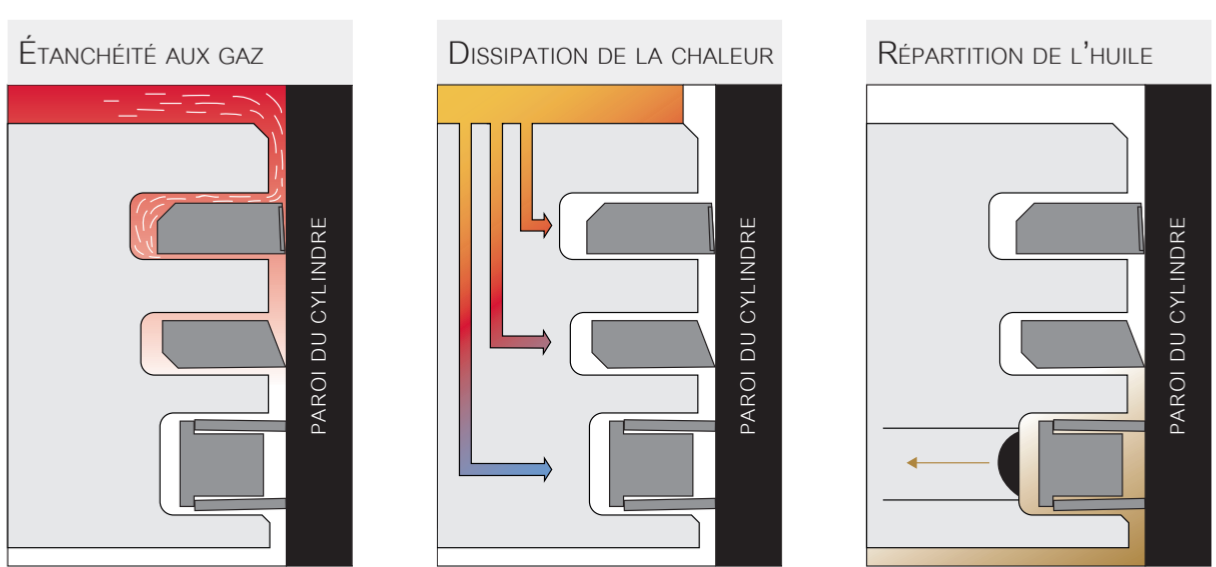
\includegraphics[width=0.7\linewidth]{Img/fonction-segment}
	\caption[Segments]{fonctionnement des segments}
	\label{fig:fonction-segment}
\end{figure}

\subsection{Lubrification du système Segment-Chemise-Piston}
Le carter a pour rôle de contenir l'huile dont le moteur a besoin pour sa lubrification. Les masses d'équilibrage du vilebrequin trempent dans l'huile du carter, pour qu'une lubrification par barbotage et projection soit assurée lors de la rotation du vilebrequin. La rotation du maneton du vilebrequin dans le carter fait qu'il y ait projection importante de la quantité d'huile à la surface de la chemise. cette huile se coulerait naturellement vers le carter si le piston ne disposé pas des segments qui poussait l'huile vers le chambre de combustion (il est aussi import de comprendre que dans un moteur qui tourne à 2000 tour la minute, le piston accomplis sa course en moins de 0,01 seconde). En effet, durant la course descendant du piston, les segments raclent effectivement l'huile mais, conformement à l'équation fondamental d'équilibre de force, la mettent sous pression. \\

L'interaction entre les segments et la chemise est décrit par le comportement tribologique le plus compliqué dans les moteurs à combustion interne.\cite{Arup} Lors du glissement du piston dans la chemise, le contact est soumis à des variations cycliques importantes et rapides de pression, de vitesse et de température. Cette variation a pour conséquence de faire balayer le contact segment-chemise par tous les régimes de lubrification. Les régimes de lubrification sont souvent illustrés par la courbe de Stribeck, illustrée dans la (figure \ref{fig:regime-de-lubrification}). Même si la courbe de Stribeck a été initialement développée pour les paliers lisses, elle est considérée comme applicable à d'autres systèmes lubrifiés.\cite{initiation} Car c'est une bonne représentation de la façon dont les régimes de lubrification dépendent de la vitesse, de la viscosité du lubrifiant et de la charge.\\

\begin{figure}[h]
	\centering
	\includegraphics[width=0.7\linewidth]{"Img/regime de lubrification"}
	\caption[Courbe de stribeck]{Regime de lubrification courbe de Stribeck \cite{initiation}}
	\label{fig:regime-de-lubrification}
\end{figure}

Dans le système SPC, les pertes par frottement proviennent de deux types de contact « jupe de piston-chemise et segments-chemise ». La contribution de chaque compartiment est schématisée dans la (figure \ref{fig:repartition-des-pertes-mecanique}), repris dans \cite{ayad2}. Si on positionne les sous-systèmes du moteur sur la courbe de Stribeck représentée sur la (figure  \ref{fig:regime-de-lubrification}), on peut observer la large gamme des pertes par frottement occupée par le contact piston-segments-chemise (Figure \ref{fig:repartition-des-pertes-mecanique}).\\

Les différents régimes de lubrification possible entre segments-chemise sont : la lubrification limite, mixte, et hydrodynamique.\cite{ayad2} 

Dans le régime hydrodynamique « au voisinage du point-milieu\footnote{Correspond au point équidistant entre le PMH et le PMB, où le piston atteint sa vitesse maximale} », la charge est supportée uniquement par le film d’huile, la totalité de la surface du segment est couverte de lubrifiant d’où un frottement quasi-inexistant ; ce régime intervient uniquement lorsque la vitesse de glissement est élevée, et la pression derrière le segment faible. Dans le régime lubrification mixte « au voisinage du PMH et PMB » : une partie du segment est seulement lubrifiée ; la charge étant supportée par le film d’huile et les aspérités des surfaces ; ce régime intervient uniquement lorsque la vitesse est faible et la pression derrière le segment élevée. Enfin, pour la lubrification limite, cas où la présence du lubrifiant est inexistante, la charge est entièrement supportée par les aspérités de surface.

\begin{figure}[h]
	\centering
	\includegraphics[width=0.7\linewidth]{"Img/Repartition des pertes mecanique"}
	\caption[Repartition des pertes dans le SPC]{Repartition des pertes dans le système SPC}
	\label{fig:repartition-des-pertes-mecanique}
\end{figure}
Des études expérimentales et théoriques sur la lubrification de l'ensemble SPC ont démontré que le régime de lubrification hydrodynamique est dominant au milieu de la course, là où la vitesse du piston est maximale et la pression et la température sont relativement faibles. En ce régime, le film lubrifiant est assez épais, permettant la séparation complète des surfaces en contact. La charge appliquée est entièrement supportée par le film et le comportement tribologique dépend uniquement des propriétés rhéologiques du lubrifiant dans la zone de contact. Aux extrémités du parcours du piston dans la chemise, point mort haut et bas, les sollicitations deviennent très sévères en raison de la combinaison de plusieurs facteurs : vitesse faible voire nulle, gradient élevé de pression et de température, manque de lubrification.\cite{Amal}\\

\begin{figure}[h]
	\centering
	\includegraphics[width=0.7\linewidth]{"Img/repartition de regime de lubrification"}
	\caption[Repartition de regime de lubrification]{Repartition de regime de lubrification dans la zone SPC}
	\label{fig:repartition-de-regime-de-lubrification}
\end{figure}

Afin de réduire le frottement et l'usure et par conséquent l'efficacité énergétique de ce contact,une lubrification optimale est recherchée. Les travaux de recherche et d'ingénierie actuels visent à établir une lubrification qui à la fois s'approche du point de fonctionnement minimisant les pertes mécaniques en frottement et qui se situe entre la lubrification en film complet et le régime mixte. De même, les stratégies d’optimisation visent, à iso-valeurs de vitesse, pression et viscosité, à décaler le régime de fonctionnement vers un régime purement visqueux, si possible dans la zone de rendement maximale.\\

Le contact segments-chemise a fait l’objet de plusieurs études et modélisation dans le régime hydrodynamique, mixe, et élastohydrodynamique. Cependant, comme l’indique la (figure \ref{fig:regime-de-lubrification}), l'augmentation des charges rend les paramètres tribologiques difficiles et amène la lubrification du contact segments-chemise à la frontière des régimes mixte et limite. Ceci se traduit par une forte contribution du frottement limite (figure\ref{fig:repartition-de-regime-de-lubrification}) qui mène à une importante augmentation de la dissipation d'énergie, il est donc essentiel de renforcer la compréhension du mécanisme de frottement dans ces régimes-là.\\

Pour répondre à la problématique de lubrification du contact SPC, plusieurs paramètres peuvent être optimisés, tel que la géométrie et les caractéristiques élastiques du segment, le matériau des surfaces en contact et les conditions de fonctionnement. Mais il y a deux leviers qui se sont montrés particulièrement intéressants et sur lesquels porteront les études effectuées dans le cadre du présent travail : l'état de surface des chemises et les propriétés du lubrifiant.\\

Les propriétés du lubrifiant représentent un paramètre d'une grande importance pour
l'amélioration des performances tribologiques des MCI. On parle notamment de l'apport des additifs ajoutés aux huiles formulées par rapport aux huiles de base. Les additifs permettent de réduire la viscosité du lubrifiant en maintenant une épaisseur suffisante de ce dernier entre les surfaces en mouvement relatif. Ils permettent également d'optimiser les propriétés chimiques du lubrifiants afin de mieux s'adapter aux conditions de fonctionnement, tout en permettant de réduire l'impact environnemental. La qualité de l'huile est ainsi l'un des éléments clés pour assurer un meilleur rendement des MCI.\\

Il apparait donc nécessaire de récapituler l'état des connaissances dans ces deux domaines clés. Ainsi, les prochaines parties présentent un état de l'art sur la topographie des surfaces et sur la composition du lubrifiant en considérant ces deux leviers comme des solutions technologiques.\\

\subsection{Influence du système SPC sur rendement moteur}
L'usage répandu du MCI dans diverses applications est dû à ses performances et à sa fiabilité. Néanmoins, son rendement énergétique est limité par des considérations thermodynamiques.\cite{kennet} En effet, l'énergie générée par la combustion du carburant et transmise au piston n’est pas tout à fait disponible sur l’axe sortant du moteur, uniquement $21.5\%$ de l'énergie effectivement libéré par la combustion est transformée en énergie utile\cite{kennet}. La (Figure \ref{fig:perte-de-lenergie-fourni})  présente la répartition de la consommation énergétique pour un véhicule fonctionnant à une vitesse de 60 km/h. Une grande partie de l'énergie est dissipée sous forme de perte thermique à l'échappement. Les pertes mécaniques par frottement sont relativement importantes, de l'ordre de $11\%$ de l'énergie libérée, soit environ un quart des pertes thermiques\cite{kennet},Dans le cadre de ce travail, on s'intéresse en particulier à l'étude comparatif des performances de la lubrification synthétique usée et éco-lubrifiant.\\

Les pertes par frottement à l'intérieur du moteur apparaissent au niveau de toutes les pièces mécaniques en mouvement relatif. Afin de les réduire et augmenter le rendement du moteur, il faut tout d'abord identifier les éléments responsables de ces pertes. La (Figure \ref{fig:perte-de-lenergie-fourni}(b)) montre une répartition typique du frottement mécanique à l'intérieur du moteur. Le système Segment-Piston-Chemise (SPC) représente le pourcentage le plus élevé (entre $38 et 68\%$).\cite{kennet} En conséquence, il apparait judicieux de s'intéresser en priorité à la réduction du frottement dans cet ensemble.\\
\begin{figure}[h]
	\centering
	\includegraphics[width=0.5\linewidth]{"Img/perte de l'energie fourni"}
	\caption[Repartition de d'éneergie]{Repartition de d'éneergie dans un moteur à combustion interne}
	\label{fig:perte-de-lenergie-fourni} \cite{Amal}
\end{figure}

Aujourd'hui, des efforts considérables sont consacrés à la production de véhicules et de machines de plus en plus efficaces et économes en énergie, non seulement pour des raisons économiques, mais aussi pour contribuer à répondre aux exigences de réduction des émissions polluantes. Les réglementations gouvernementales, de plus en plus strictes, exigent une économie de carburant et des émissions réduites comme L'Environmental Protection Agency (EPA) impose des normes sur les émissions des véhicules légers, ciblant une réduction constante des émissions de CO₂. Pour les modèles 2023, la consommation moyenne de carburant a atteint un record de 27,1 miles par gallon, avec une réduction des émissions réelles de CO₂ à 319 grammes par mile. Les véhicules électriques et hybrides jouent un rôle croissant, représentant $11,5\%$ de la production en 2023 et atteignant $14,8\%$ en 2024. Ces avancées s'inscrivent dans des efforts de longue date visant à réduire les émissions des véhicules de près de $31\%$ depuis 2004, tout en améliorant l'efficacité énergétique de $40\%.$ \cite{epa}\\

L'industrie automobile doit faire face est l'épuisement progressif des ressources pétrolières, entraînant une augmentation significative de leur coût. Cette réalité accentue la nécessité de réduire la consommation énergétique des véhicules, en mettant l'accent sur des solutions visant à diminuer la consommation de carburant.\\

Des véhicules économes en carburant et amis de l'environnement ont fait objet de plusieurs travaux de recherche. De nombreuses solutions techniques ont été mises en place, mais l'amélioration du rendement des MCI via la réduction des pertes mécaniques en frottement est toujours un sujet d'actualité.\cite{Amal} Par conséquent, l’étude du contact SPC trouve ici tout son intérêt.\\


En résumé, bien que les moteurs à combustion interne soient essentiels à de nombreuses applications, leur rendement reste limité par des contraintes thermodynamiques. Une grande partie de l'énergie est perdue sous forme de chaleur et de frottement. Ces limites énergétiques rendent cruciales les recherches sur la réduction des pertes mécaniques, afin d'améliorer l’efficacité des moteurs actuels

\section{\textsc{Etat de l'art}}\label{etat_art}
Durant cette section, nous allons mettre en lumière quelques études précédemment menées, par des chercheurs, dans les domaine de la tribologie et la lubrification en générale et de l'ensemble Segment - Pyston - chemise (SPC) en particulier. Depuis 1880 av J-C en Égypte passant par la révolution industrielle aux alentours de 1760, jusqu'à nos jours, les avancés dans ce domaines cité ci-haut sont énorme, ainsi nous aurons le plaisir d'y naviguer dans la suite.
\subsection{Perspective historique}
L’histoire de l'invention et l'utilisation des segments remonte à bien loin avant la révolution industrielle. Les Grecs aux alentours de 250 avant J.C., ont été les premiers à employer un système qui scelle un cylindre pour soulever de l'eau. Cependant, le développement de telles machines a été abandonné pendant le moyen âge, et la technologie du système piston-cylindre n'a pas été reprise qu'au 17siècle. Repris dans \cite{ayad2}.

De grandes avancées ont été réalisées pendant le développement du moteur à vapeur, James WATT a boulonné une matrice de chanvre étroitement attachée au piston afin d'empêcher la fuite des gaz à haute pression. Ce n'était qu'en 1797 que le Révérend Edward CARTRIGHT a proposé l'utilisation des anneaux métalliques au lieu de la garniture court-durable de chanvre. Cependant, les ensembles devenus plus complexes impliquaient en général le montage de ressorts pour assurer une bonne étanchéité. Dans la moitié du 19 siècle, John RAMSBOTTOM a proposé un modèle simple et ingénieux qui éliminerait tout le besoin des assemblages complexes déjà utilisés. Sa conception consistée en un anneau de diamètre plus grand de $10\%$ que le diamètre du cylindre en lequel il serait installé, tout en utilisant sa propre élasticité pour sceller l'interface du cylindre \cite{ayad2}.

Durant les années 20, les anneaux métalliques de Ramsbottom ont été employés intensivement, et il n'y avait pas de besoin réel de développement en raison des conditions de fonctionnement simple et basique. Cependant, avec le développement et la progression des vitesses et des charges, la consommation d’huile et le transfert thermique posaient de plus en plus de problèmes dans un environnement de plus en plus dur. Des efforts étaient donc nécessaires pour optimiser la conception des anneaux de Ramsbottom dans un but de minimiser le frottement et l’usure. Des études plus détaillées sur le frottement et la lubrification des segments ont ainsi commencés \cite{ayad2}.

\subsection{Modelisation de la lubrification et du frottement}
Une évolution substantielle a été faite par les chercheurs durant les décennies passées, et qui a mené à une meilleure compréhension du comportement des segments et de leur effet sur le fonctionnement du moteur. L’application de la théorie hydrodynamique de lubrification aux segments a été utilisée pour la première fois par Castleman en 1936\cite{stephen}. Une grande progression a été faite pour modeler numériquement et obtenir la variation cyclique de l'épaisseur de film d'huile par Furuhama\cite{ayad2}, avec la considération d’une vision plus réaliste de la course du segment, le profil de surface et les effets des pressions des gaz Blow-By. Par la suite, une analyse complète a été faite dans le travail de Dowson avec l'application de conditions aux limites plus réalistes. Les contributions les plus importantes de cette référence sont : 1ere condition d’entrée appliquée en considérant différentes sources d'huile pour différents segments, et 2eme condition de sortie (condition de Reynolds) est appliquée pour la lubrification hydrodynamique. L'effet de la forme du segment sur l'épaisseur de film d'huile a été aussi considéré et s'est avéré très significatif.\\

Par la suite, plusieurs modèles et études ont vu le jour ayant comme axe de recherche : les différents régimes de fonctionnement du moteur, les différentes caractéristiques des segments et des chemises, le type de lubrification, le frottement, l’usure et l’épaisseur du film d'huile Akalin et Newaz ont proposé un modèle qui simule le contact segments-chemise en lubrification mixte. Les résultats trouvés comparés avec des résultats expérimentaux montrent que l’essentielle du cylindre se trouve en régime de lubrification hydrodynamique. Néanmoins, le coefficient de frottement subit une légère augmentation aux PMB et PMH, et cela en raison du passage d’un régime hydrodynamique à un régime mixte. Quelques chercheurs ont également développé des modèles uni et bidimensionnel, en se concentrant sur les effets de la déformation du cylindre, la dynamique des segments, la géométrie du segment, l'épaisseur de film d'huile et des écoulements des gaz Blow-By \cite{Amal}\cite{Arup}\cite{ayad1}.\\

Taylor et son équipe étaient les premiers à faire une étude sur les effets du taux de cisaillement des couches d'huiles sur le frottement et l'épaisseur du film d'huile. Les prévisions de leur modèle unidimensionnel ont été également comparées aux mesures expérimentales de l'épaisseur du film d'huile pour différents types de lubrifiants. D'excellents résultats ont été obtenus, qui démontrent qu’un modèle unidimensionnel convient à étudier le frottement et les effets des types des huiles sur le contact segments-chemise\\

Dans les modèles de lubrification du contact segments-chemise, plusieurs hypothèses simplificatrices sont généralement faites. Le lubrifiant est souvent considéré comme Newtonien. Néanmoins, il existe des modèles plus complet et sophistiqués pour lesquels la viscosité varie avec les contraintes de cisaillement\cite{tribo1}\cite{trobo2}. Des études sur le transport de l’huile dans le système segments-piston-chemise ont été aussi menées par Gamble , Thirouard, Stark, où ils présentent son influence sur l’épaisseur minimale de film d’huile. Il existe aussi des techniques qui permettent de visualiser le transport d’huile et mesurer l’épaisseur du film lubrifiant\cite{tribo1}.\\

Des conditions aux limites variées sont utilisées pour les modèles de simulation. Les conditions de Sommerfeld permettent des valeurs de pression positives aussi bien que négatives. Les conditions de Swift-Steiber en revanche désignent les régions de pression négative comme zone de cavitation où la pression est nulle. Plusieurs études ont proposé de nouvelles conditions aux limites, avec des modèles prenant en compte le phénomène de cavitation et de rupture du film d’huile\cite{trobo2}.

\subsection{La texturation de surface}
la rugosité des surfaces est un des éléments clé pour la réduction du frottement et de l’usure ; elle a bénéficié d’une attention particulière dans la littérature spécialisée. Une bonne façon de relater son histoire se trouve dans l’étude de Masuzawa et Etsion \cite{ayad2}. \\

Le frottement entre les segments et la chemise est en fonction de la charge, la topographie des surfaces et la lubrification du contact qui elle, est liée à la viscosité de l’huile.Rohde était le premier à proposer un modèle de lubrification mixte pour les segments, en utilisant le modèle d’équation de Reynolds en régime mixte établi par Pâtir et Cheng, des conditions aux limites de Sommerfeld, et un modèle de contact de surface rugueuse Greenwood-Tripp\cite{initiation}.Son modèle a étudié l’effet de la rugosité des surfaces et l'orientation des aspérités sur le frottement entre les segments et la chemise, un contact dur des aspérités a été détecté aux extrémités de la course, particulièrement autour du PMH lors de la compression/explosion, où la pression élevée des gaz donne une charge radiale supplémentaire sur le segment supérieur. Il a également constaté qu’une augmentation de la surface de rugosité augmente non seulement la magnitude des aspérités mais également la perte de puissance par frottement, en outre, l'orientation de la rugosité et la différence entre un segment rugueux/chemise lisse et un segment lisse/chemise rugueuse ont été revue.\cite{tribo1}\\

Dans le modèle de Sui et Ariga qui prend en considération la topographie de la chemise dans un mode de lubrification mixte, des résultats de simulation ont été comparés aux résultats expérimentaux. Ces résultats montrent une possibilité de réduction du frottement atteignant les $9\%$ par une modification de l’orientation des aspérités de la texture. Selon cette étude, l’épaisseur du film lubrifiant entre le segment coupe-feu et la chemise est en moyenne peu influencée par la texture, d’où les changements en frottement aussi. Cependant, ce segment subit les frottements les plus importants par rapport au deux autres, et cela est dus principalement à un contact plutôt limite qu’hydrodynamique ou mixte avec la chemise. Quant aux segments d’étanchéité et racleur, l’étude montre en revanche que les valeurs du frottement sont différentes selon la texture utilisée. repris dans \cite{ayad2}\\

La microgéométrie de la surface de la chemise joue un rôle très important dans les pertes par
frottement et dans la consommation de l’huile dans un moteur à combustion interne. Une
des texturations classiques de cette surface est celle créée par pierrage. Une étude Hafedh BOUASSIDA a permis d'écrire un modèle simplifié du contanct Segment chemise en présence de la microgéométrie. Puis, un code de calcule basé sur la méthode numérique multigrille a été développé. Les r´esultats mettent en évidence deux mécanismes distincts de génération de portance selon le type du segment.\cite{hafedh}\\

Tout au long de ce chapitre nous avons appréhendé quelques notions de bases dans la compréhension de notre travail notamment:le   moteur à combustion interne à mouvement alternatif, le système SPC.On peut donc apercevoir que l’étude du triplet segments-chemise est passionnante et présente un intérêt majeur, malgré les résultats divergents et incohérents de temps à autre. Les avancées scientifiques actuelles sur ce sujet présentent un consentement sur l’utilisation de la texturation pour une importante réduction du frottement et perte de charge. 